%%%%%%%%% begin snippet
%% You need to add the package "tabularx".
%% Place the snippet right after \begin{document}

% need tabularx

\documentclass[11pt,a4paper]{article}
\usepackage{tabularx}
\usepackage{commath}
\usepackage{amssymb}
\usepackage{graphicx}
\usepackage{subfig}

\begin{document}


\begin{titlepage}
       \begin{center}
             \begin{huge}
           %% Update assignment number here
                   \textbf{Assignment 2}
             \end{huge}
       \end{center}

       \begin{center}
             \begin{large}
                   Computational Intelligence SEW, SS2018
             \end{large}
       \end{center}

       \begin{center}
 \begin{tabularx}{\textwidth}{|>{\hsize=.33\hsize}X|>{\hsize=.33\hsize}X|>{\hsize=.33\hsize}X|} 

                   \hline
                   \multicolumn{3}{|c|}{\textbf{Team Members}} \\
                   \hline
                   Last name & First name & Matriculation Number \\
       \hline
                   Hohensinner & Richard & 00273237 \\
                   \hline
                   Kim & Sathearo & 01430376 \\
                   \hline
                   Kofler & Lorenz & 01430321 \\
                   \hline

             \end{tabularx}
       \end{center}

\end{titlepage}

\section{Regression with Neural Networks}
\subsection{Simple Regression with Neural Networks}
\subsubsection*{a) Learned function}
The first three figures show the results by using a different number of neurons in a single hidden layer (including predicted output function, testing and training data).\\
As we can see in Figure 1, a number of 2 hidden neurons results in an underfitting model. It is definitely not possible to fit the output function.\\
By using 8 hidden neurons (Figure 2) it is reached a better result but it is still underfitting. With 40 hidden neurons the results are best. It seems that this amount of hidden neurons leads to almost seeming to overfit (e.g. between -1.0 and -0.5).

\begin{figure}[!htbp]
	\centering
        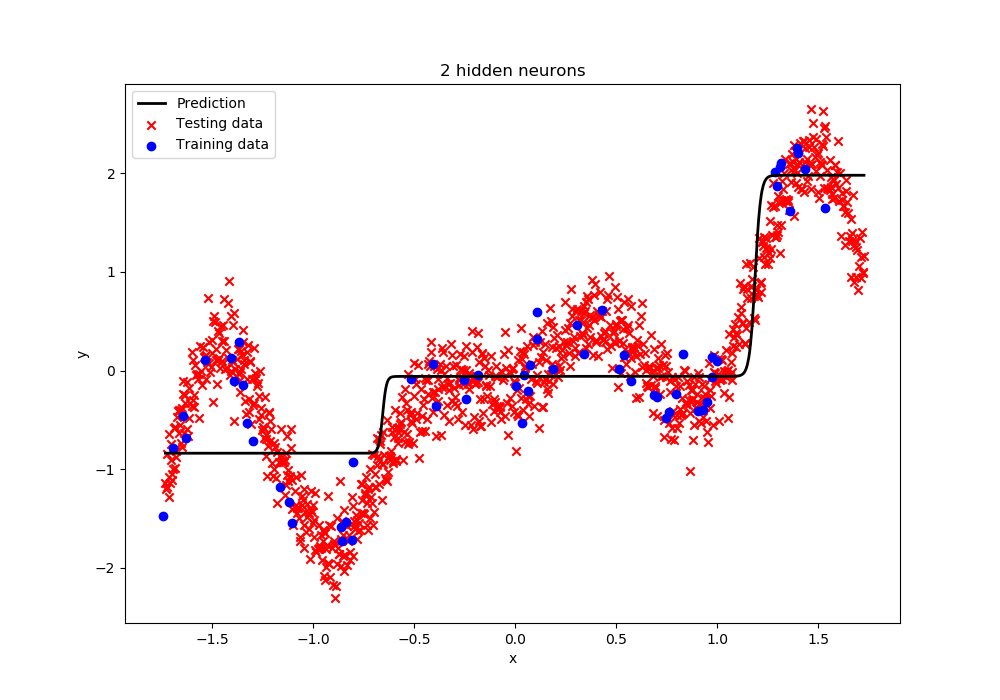
\includegraphics[width=12cm]{1_1_a_2}
	\caption{2 hidden neurons}
\end{figure}

\begin{figure}[!htbp]
	\centering
        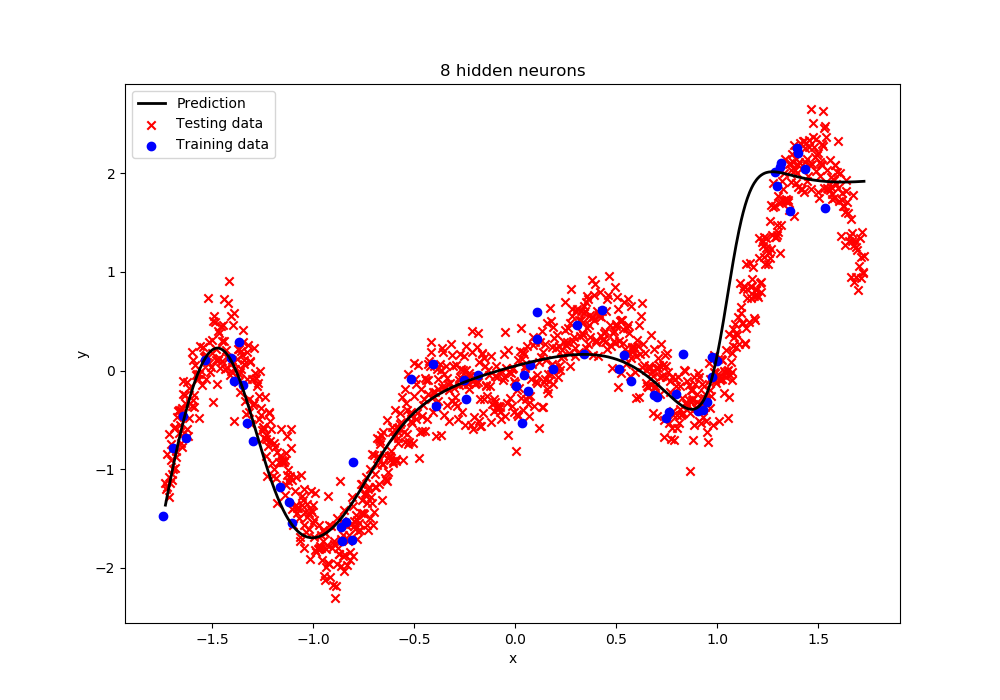
\includegraphics[width=12cm]{1_1_a_8}
	\caption{8 hidden neurons}
\end{figure}

\begin{figure}[!htbp]
	\centering
        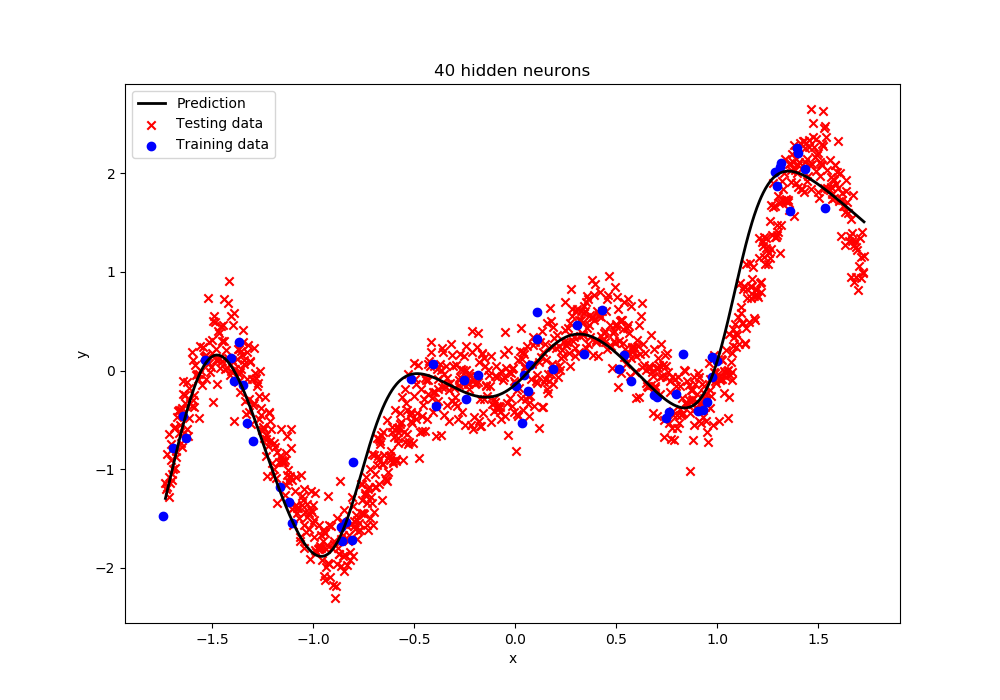
\includegraphics[width=12cm]{1_1_a_40}
	\caption{40 hidden neurons}
\end{figure}
\newpage
\subsubsection*{b) Variability of the performance of deep neural networks}
Here are the results of the training set:
\begin{itemize}
\item Minimum: 0.04443679
\item Maximum: 0.07666421
\item Mean: 0.05497159066069205
\item Standard Deviation: 0.009648747344143687
\end{itemize}
Even if they are not asked, here are the results of the test set:
\begin{itemize}
\item Minimum: 0.11682291
\item Maximum: 0.32886157
\item Mean: 0.1956105516802004
\item Standard Deviation: 0.06109058959323914
\end{itemize}
Yes, the seeds are the same at number 3.\\\\
Because there is a high difference between the deviations of the errors, it is quite dangerous to use the test set as it is. So there is a validation set needed to be sure. It is best to to use the seed that results in the lowest validation error.\\\\
Neural networks use cost functions that are not convex as they have many local minima. In contrast to, linear regression and logistic regression have convex cost functions (convergence is constant).\\\\
In Stochastic Gradient Descent the weights are updated after each training point (online learning), so the randomness is introduced. Even if it is replaced by Standard Gradient Descent there is some randomness as the initial weights are random.

\subsubsection*{c) Varying the number of hidden neurons}
As we can see in Figure 4, the best value of $n_h$ is reached at value 4. At this point, the MSE is very low and also the variance is also quite low. A lower number of hidden neurons yield a result that is not as good as the result reached at value 4. Also increasing the number of hidden neurons does not improve the results. As we have discussed within the lecture, increasing the iterations does not yield a better result. Considering the computation time the result it is also not worth to increase the number of iterations. Compared to Figure 6, where 1000 iterations were used, this variant seems to be better. Here the best value of $n_h$ seems to be around 20 as increasing the number of neurons does not give a better result but more effort.\\\\
It seems that increasing the number of neurons leads to overfitting.
\begin{figure}[!htbp]
	\centering
        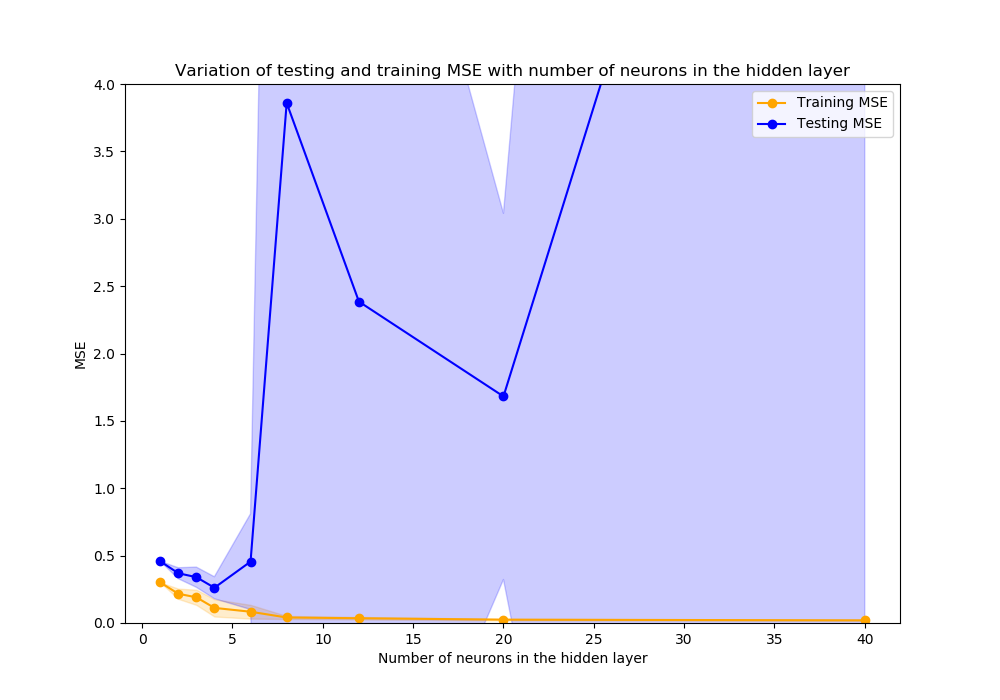
\includegraphics[width=14cm]{1_1_c_1}
	\caption{10000 iterations}
\end{figure}

\begin{figure}[!htbp]
	\centering
        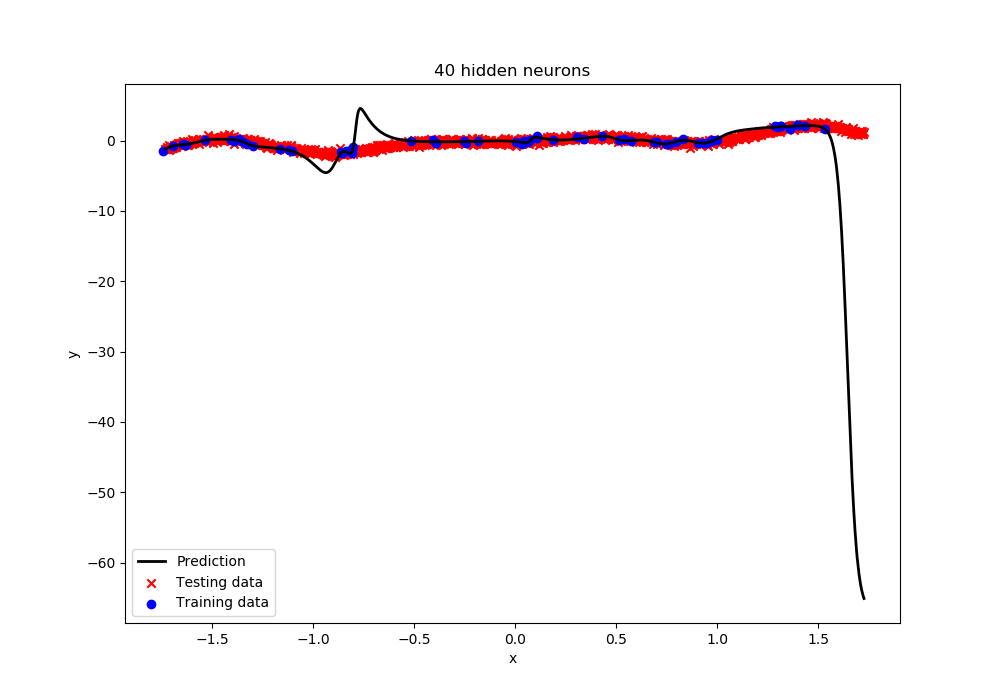
\includegraphics[width=14cm]{1_1_c_2}
	\caption{10000 iterations with 40 hidden neurons}
\end{figure}

\begin{figure}[!htbp]
	\centering
        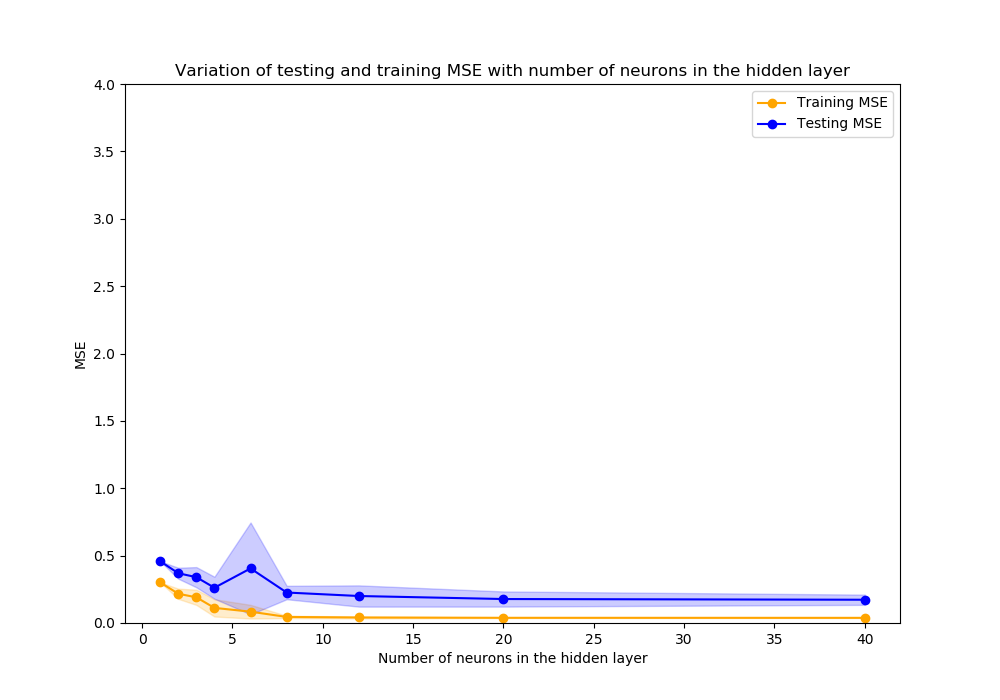
\includegraphics[width=14cm]{1_1_c_1_1000}
	\caption{1000 iterations}
\end{figure}

\begin{figure}[!htbp]
	\centering
        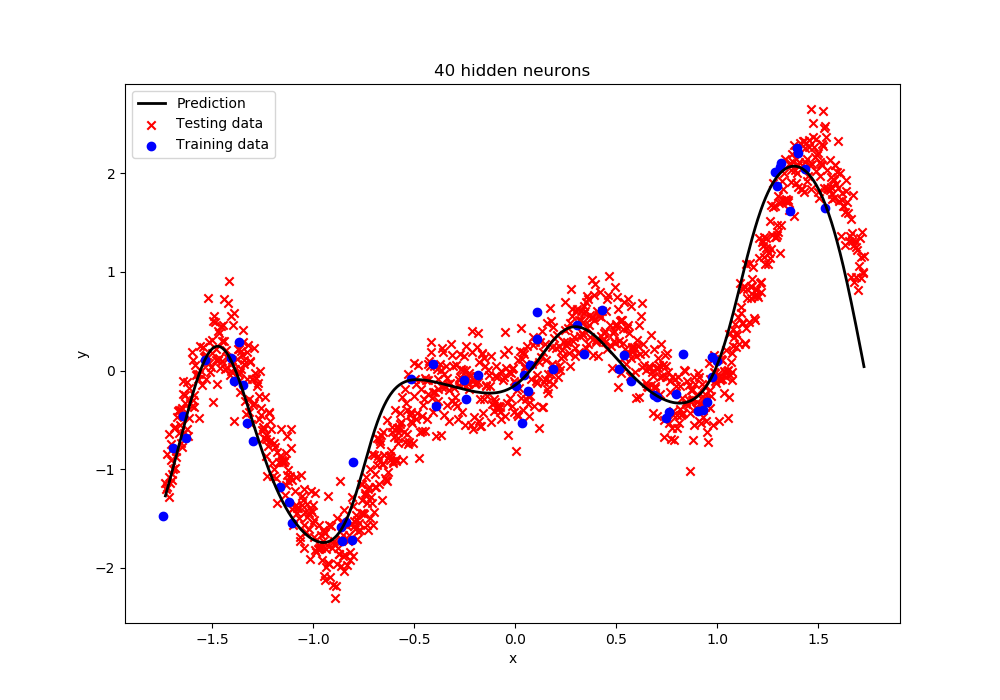
\includegraphics[width=14cm]{1_1_c_2_1000}
	\caption{1000 iterations  with 40 hidden neurons}
\end{figure}

\newpage

 \subsubsection*{d) Variations of MSE during training}
The risk of overfitting seems to increase with the number of hidden neurons. Interestingly, the overfitting exists not from a specific value on as there are some short periods where overfitting occurs and then converges again (e.g. see Figure 9 at around 1500 iterations and 8 hidden neurons). \\\\
Regarding the best solver lbfgs seems to do best (on average lowest MSE values). Above all sgd performs not as good as the other two methods.\\\\
Stochastic Gradient Descent overcomes overfitting because of the noise in the gradient. It helps to jump to probably better, new local minima.\\\\
It seems that lbfgs is better with an increasing number of neurons. It does not only use gradients (second order method). Furthermore, it converges faster.

\begin{figure}[!htbp]
	\centering
        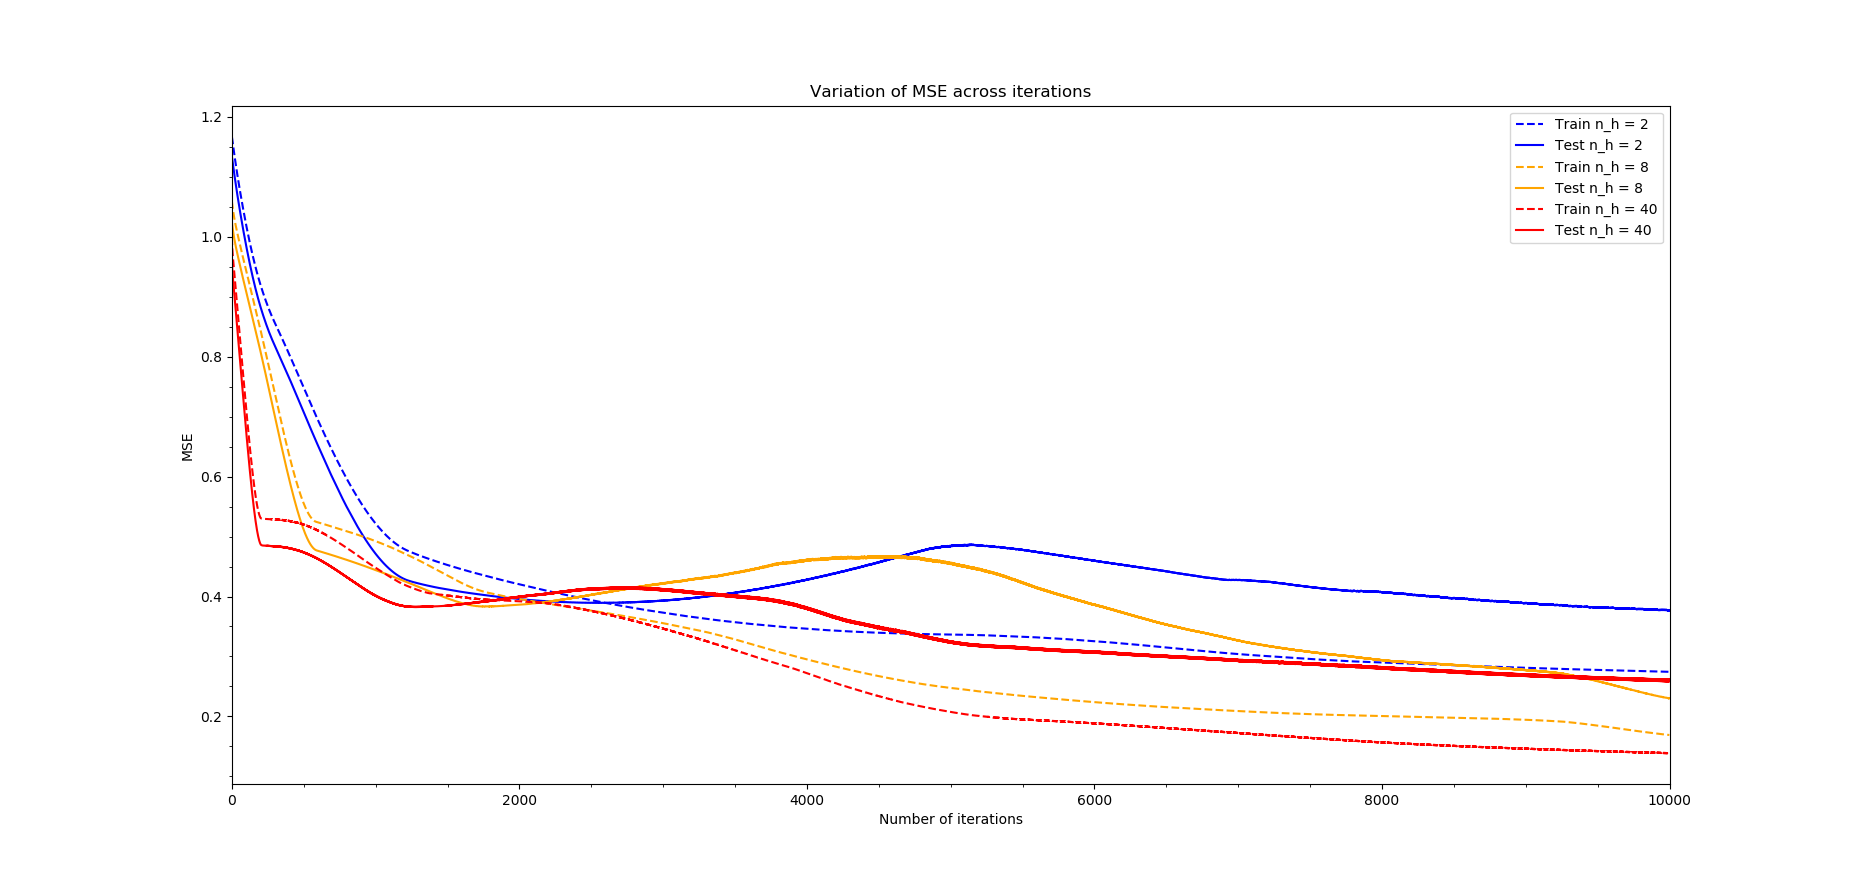
\includegraphics[width=14cm]{1_1_d_adam_rs0}
	\caption{adam}
\end{figure}

\begin{figure}[!htbp]
	\centering
        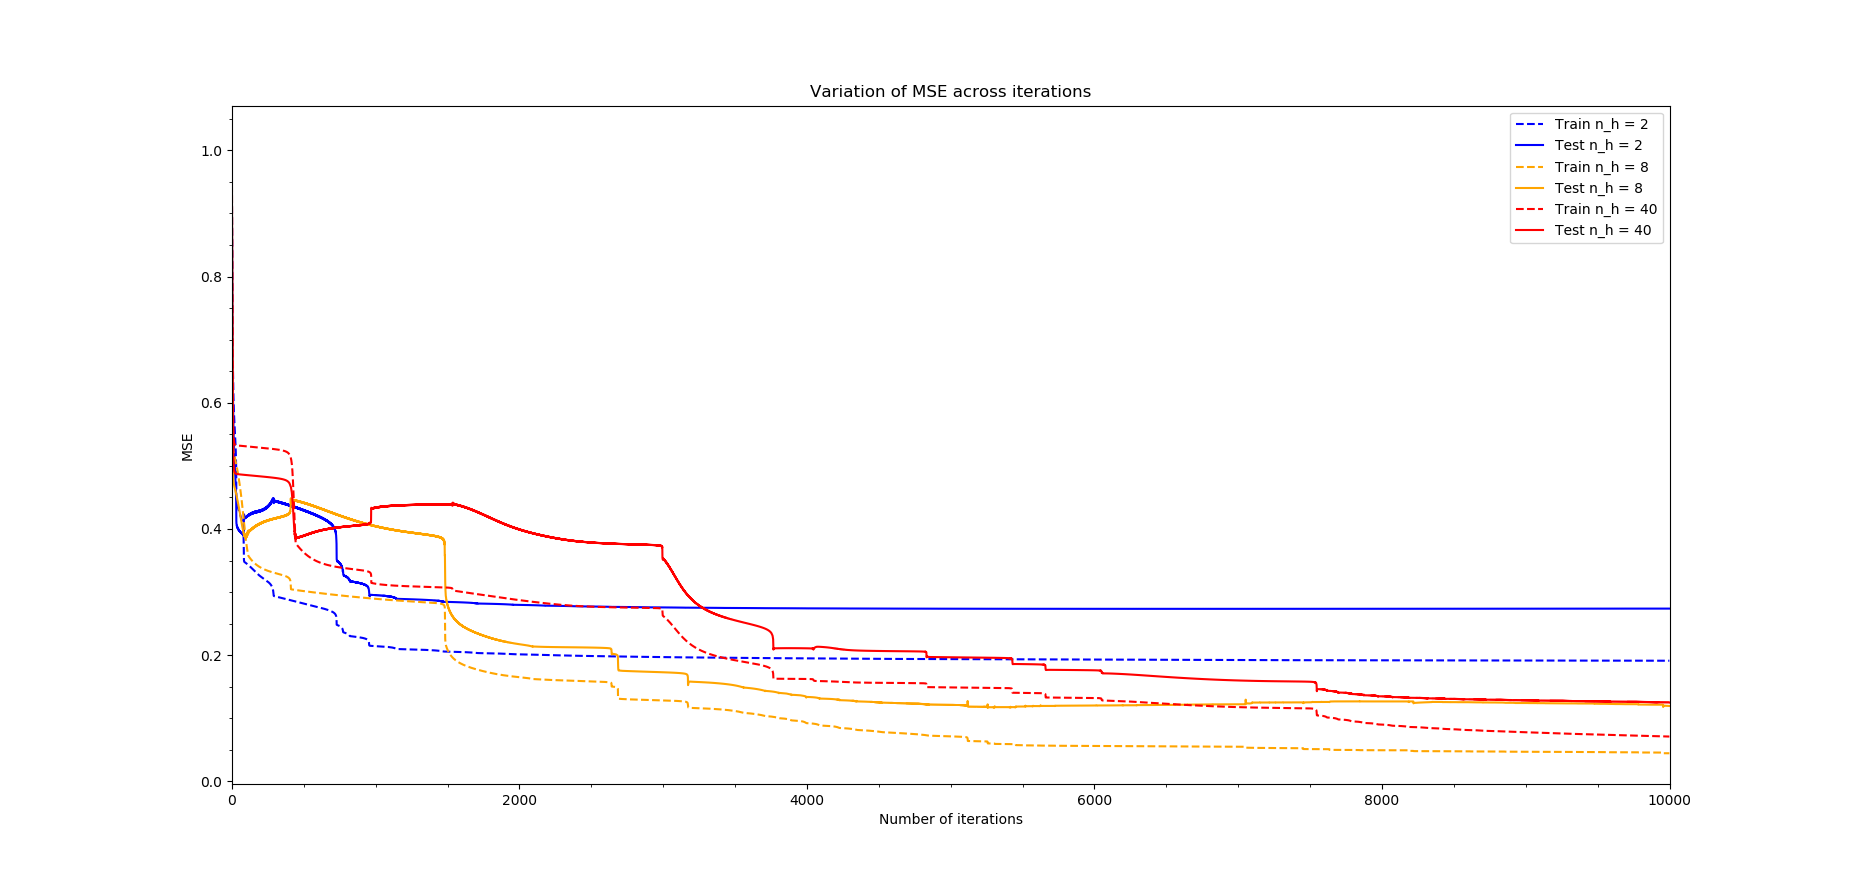
\includegraphics[width=14cm]{1_1_d_lbfgs_rs0}
	\caption{lbfgs}
\end{figure}

\begin{figure}[!htbp]
	\centering
        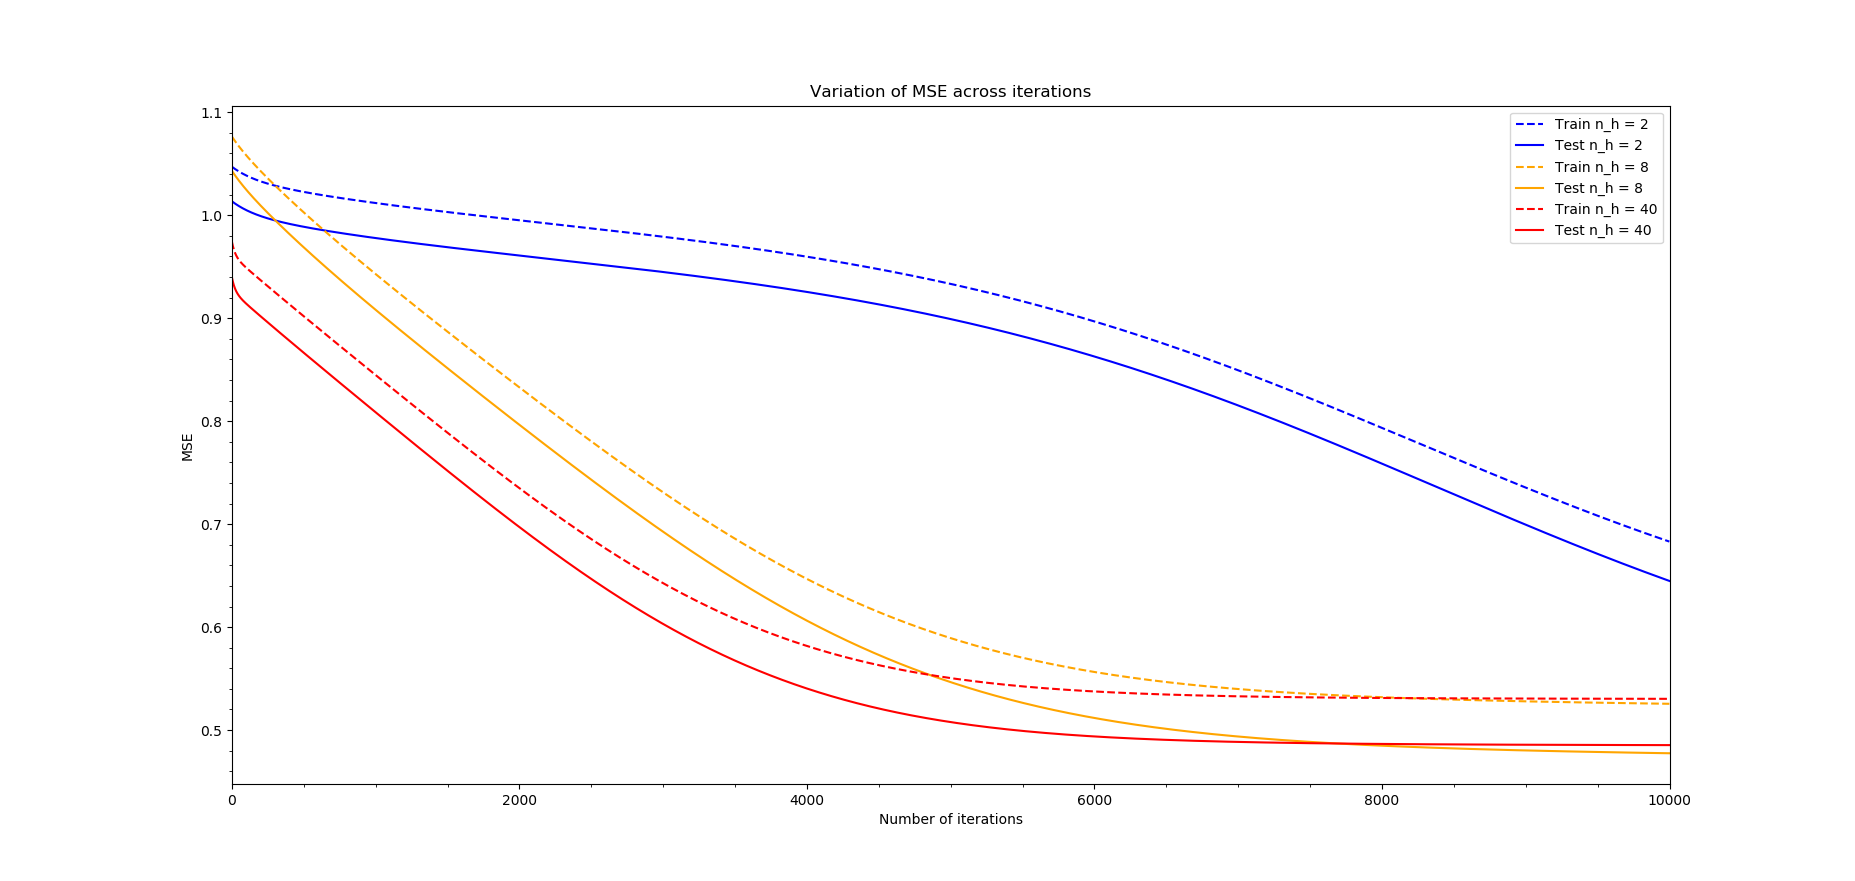
\includegraphics[width=14cm]{1_1_d_sgd_rs0}
	\caption{sgd}
\end{figure}

\newpage

\subsection{Regularized Neural Networks}

\subsubsection*{a) Weight Decay}
Figure 11 shows the dependency of the regularization parameter $\alpha$ which is best at a value of $10^{-3}$. It helps to overcome overfitting. Its main usage is to simplify the neural network and to keep the weights as low as possible.
\begin{figure}[!htbp]
	\centering
        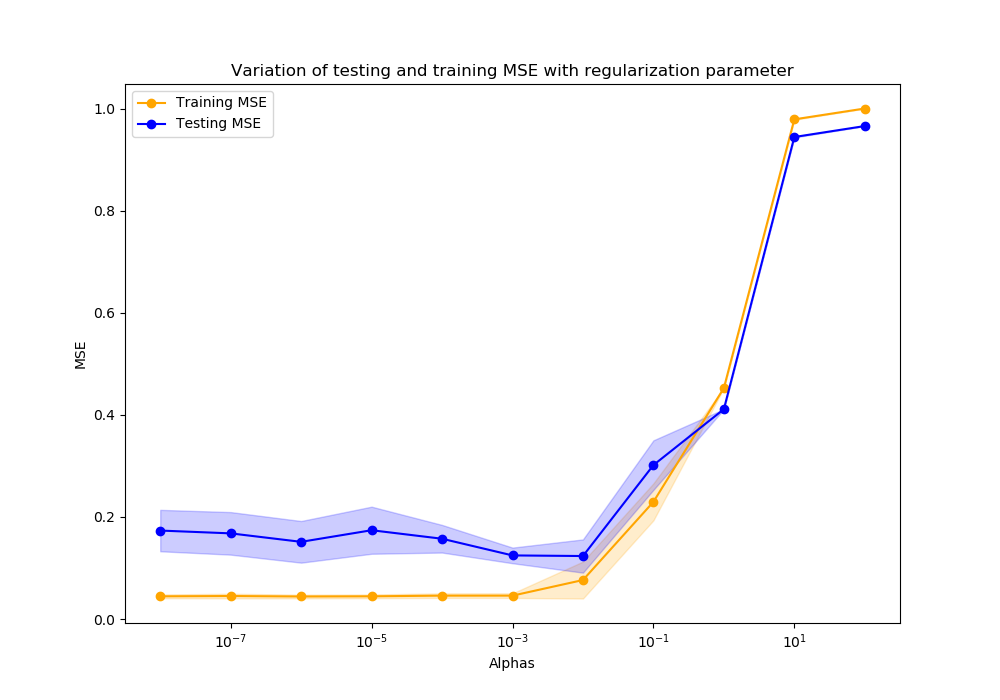
\includegraphics[width=14cm]{1_2_a}
	\caption{}
\end{figure}

\subsubsection*{b) Early Stopping}
\begin{figure}[!htbp]
	\centering
        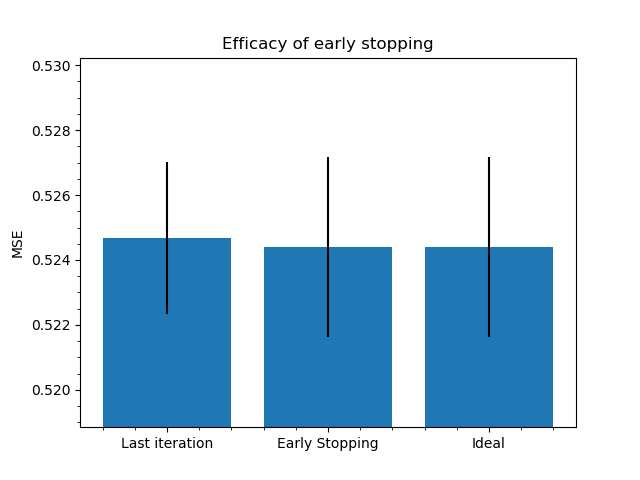
\includegraphics[width=10cm]{1_2_b}
	\caption{}
\end{figure}

\begin{figure}[!htbp]
	\centering
        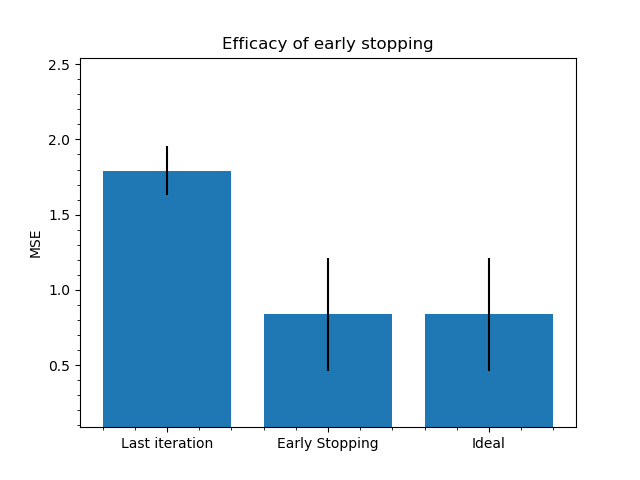
\includegraphics[width=10cm]{1_2_b2}
	\caption{}
\end{figure}

\begin{figure}[!htbp]
	\centering
        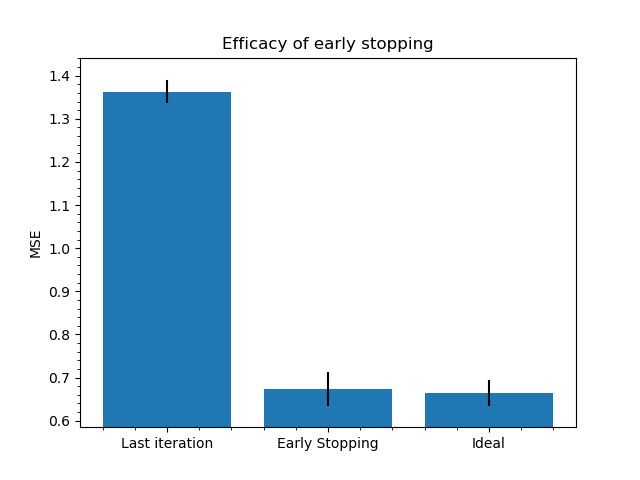
\includegraphics[width=10cm]{1_2_b4}
	\caption{}
\end{figure}
The initial values are always different because of the random seeds, so the iteration numbers will vary for random seeds. This assumption seems to be true in our case.\\\\
The standard form of early stopping is much faster. On the one hand, the problem of the used method is that the whole data must be explored so the efficiency suffers from that. On the other hand, it can overcome local minima.\\\\
As we can see in Figures 12 to 14, where some examples are plotted, the efficiency of early stopping is (almost) ideal.
\newpage
\subsubsection*{c) Combining the tricks}
-

\section{Face Recognition with Neural Networks}

\subsection{Pose Recognition}

As we can see in Figure 15, straight and up leads to misclassifications. On the other side, it works best for poses left and right.
\begin{figure}[!htbp]
	\centering
        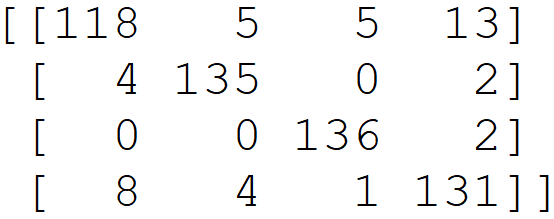
\includegraphics[width=7cm]{2_1_cfm}
	\caption{confusion matrix with rows (top to down) and columns (left to right) straight, left, right and up}
\end{figure}
\newpage
Considering Figure 16, it seems that the regions within the face are the interesting ones (above all the regions around the nose, forehead, mouth with chops and the neck are white coloured and so they get more weight).

\begin{figure}[!htbp]
	\centering
        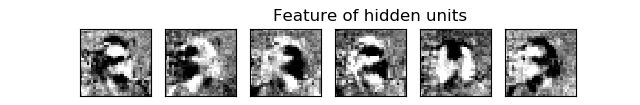
\includegraphics[width=14cm]{2_1_hidden_weights}
	\caption{hidden weights}
\end{figure}

\subsection{Face Recognition}

Random initial weights lead to different classifcations as features get weighted differently. With different initial weights also the accuracy changes as can be seen in the next ten pictures after Figure 17. The testing accuracy ranges between 0.92 and 0.96. The training accuracy is always at 1.0.

\begin{figure}[!htbp]
	\centering
        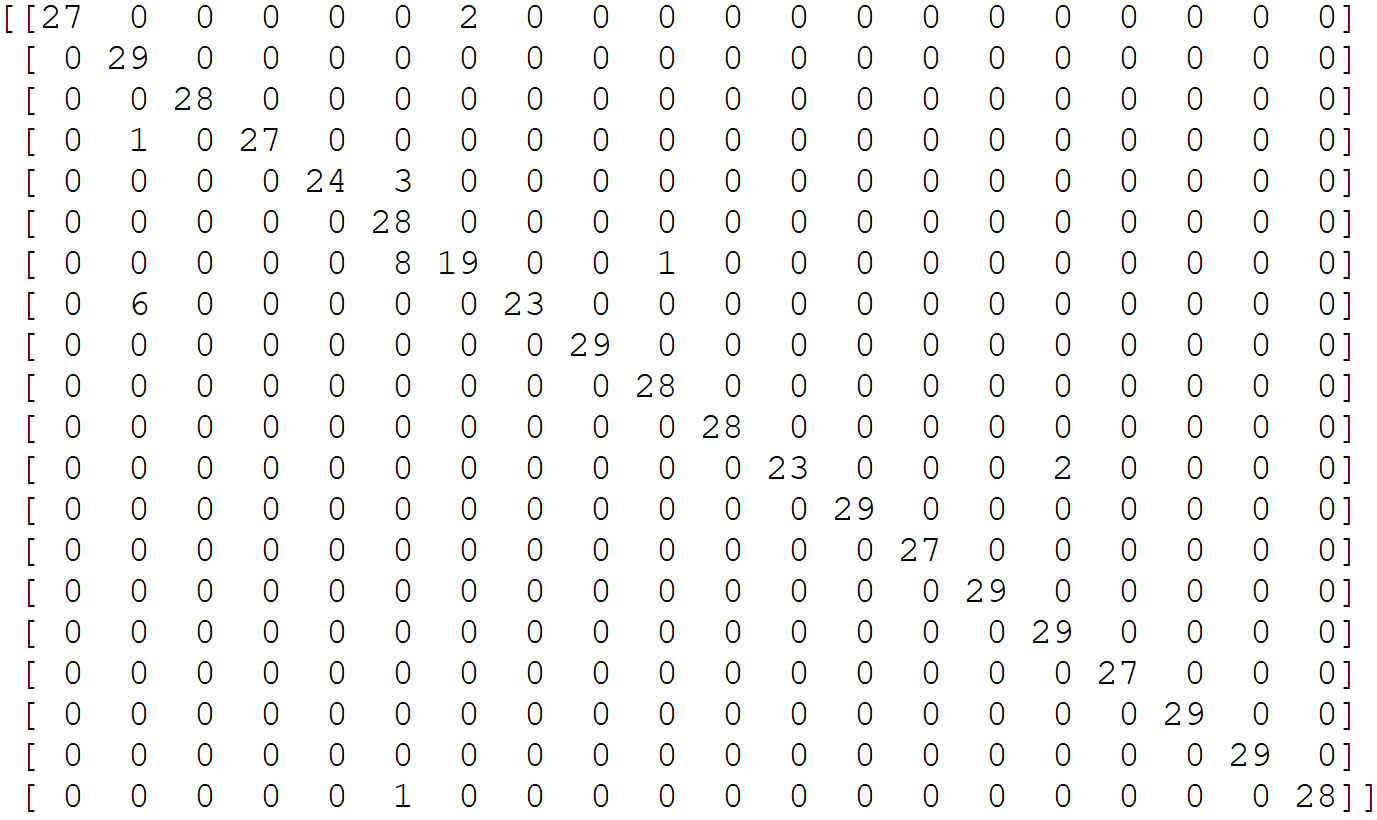
\includegraphics[width=14cm]{2_2_cfm}
	\caption{confusion matrix}
\end{figure}

\begin{figure}%
    \centering
    \subfloat[]{{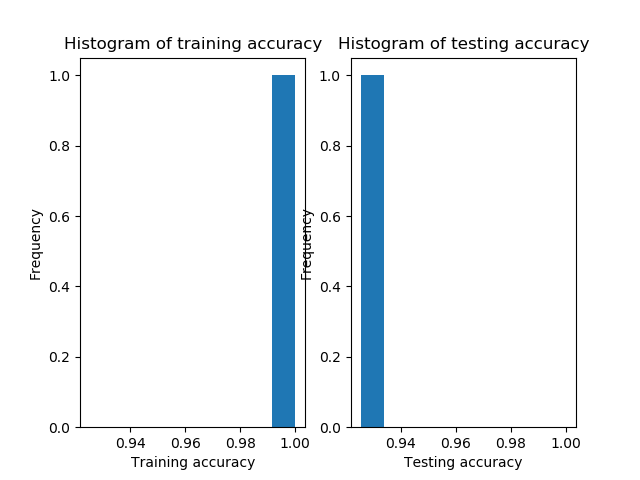
\includegraphics[width=7cm]{2_2_h01} }}%
    \subfloat[]{{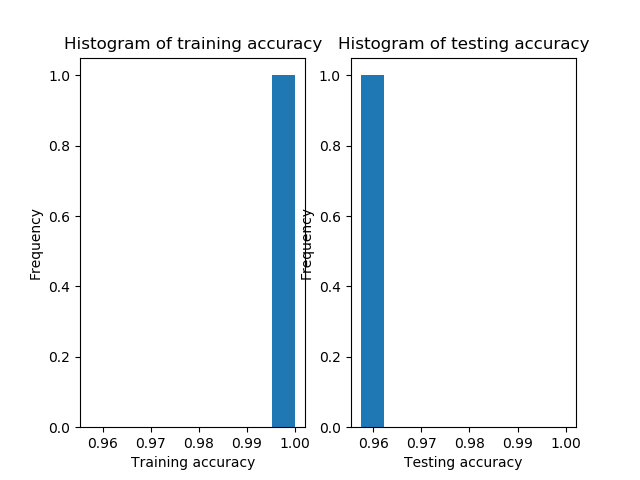
\includegraphics[width=7cm]{2_2_h02} }}%
    \caption{}%
    \label{fig:example}%
\end{figure}

\begin{figure}%
    \centering
    \subfloat[]{{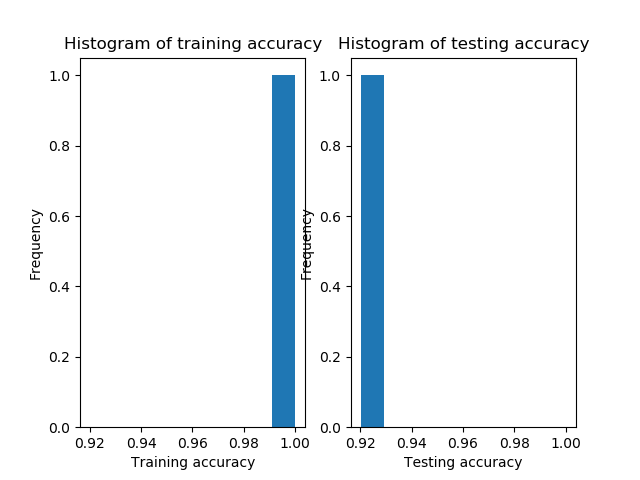
\includegraphics[width=7cm]{2_2_h03} }}%
    \subfloat[]{{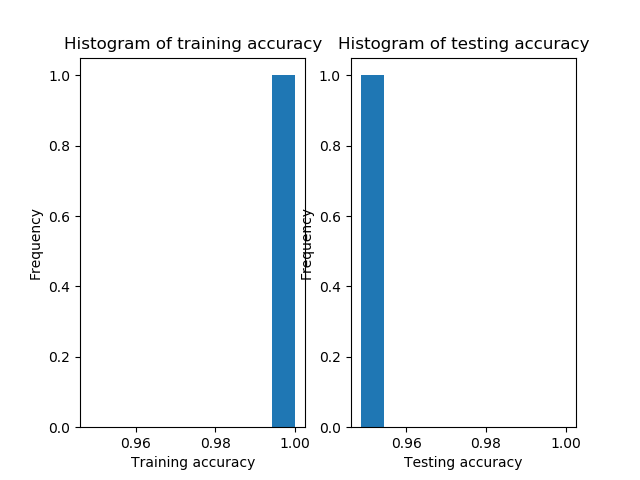
\includegraphics[width=7cm]{2_2_h04} }}%
    \caption{}%
    \label{fig:example}%
\end{figure}
\begin{figure}%
    \centering
    \subfloat[]{{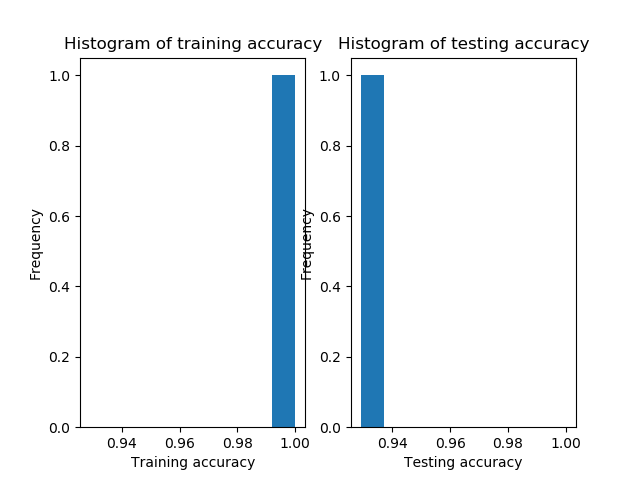
\includegraphics[width=7cm]{2_2_h05} }}%
    \subfloat[]{{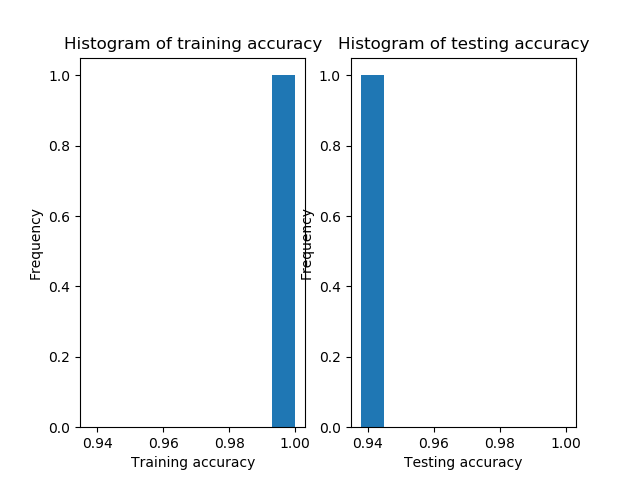
\includegraphics[width=7cm]{2_2_h06} }}%
    \caption{}%
    \label{fig:example}%
\end{figure}
\begin{figure}%
    \centering
    \subfloat[]{{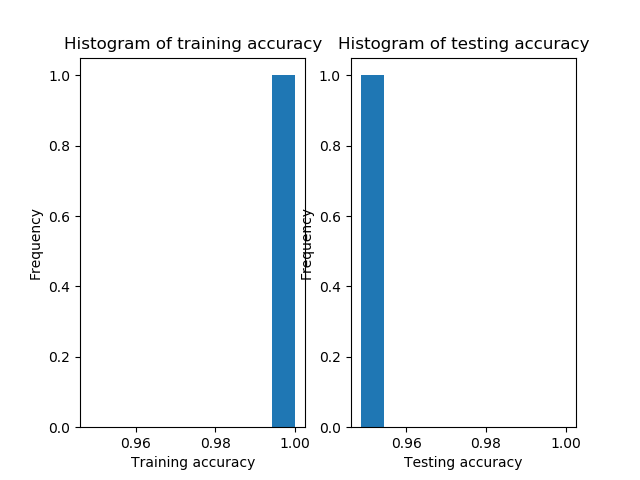
\includegraphics[width=7cm]{2_2_h07} }}%
    \subfloat[]{{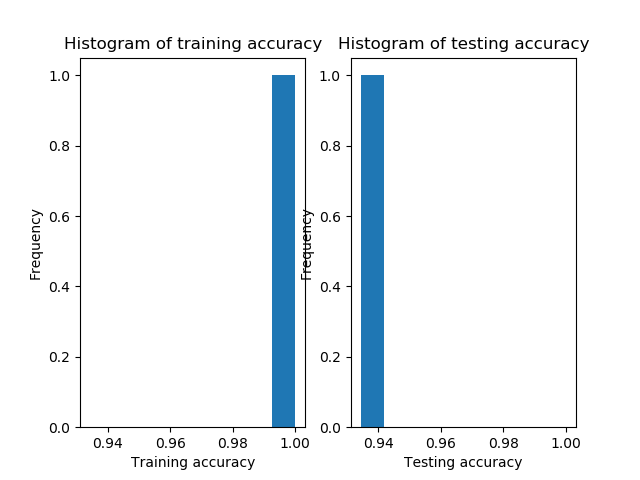
\includegraphics[width=7cm]{2_2_h08} }}%
    \caption{}%
    \label{fig:example}%
\end{figure}
\begin{figure}%
    \centering
    \subfloat[]{{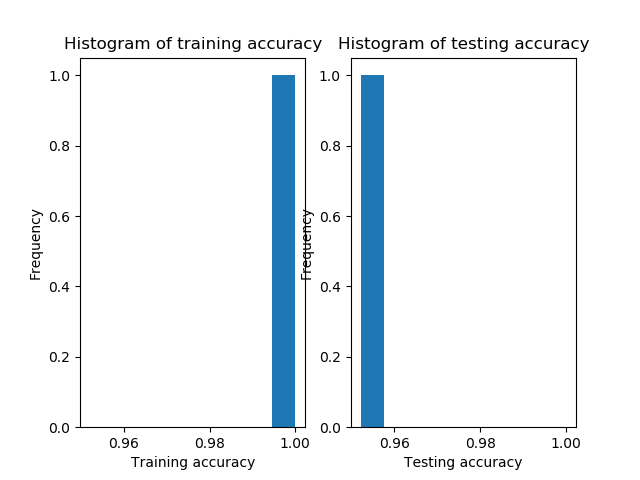
\includegraphics[width=7cm]{2_2_h09} }}%
    \subfloat[]{{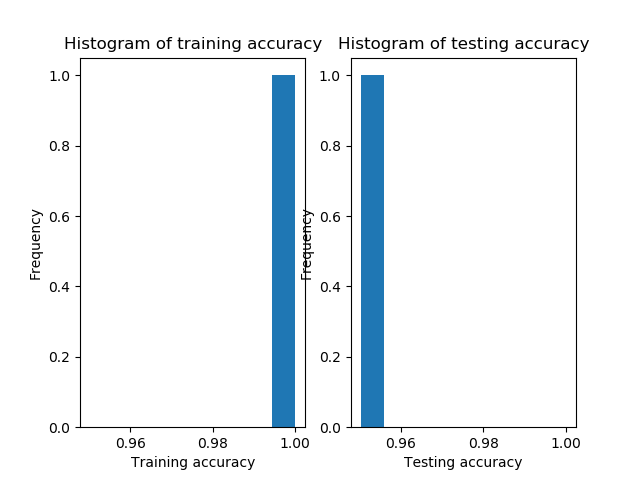
\includegraphics[width=7cm]{2_2_h10} }}%
    \caption{}%
    \label{fig:example}%
\end{figure}
\newpage
If we look at the misclassified images, we can see, that the people are looking straight forward, sometimes even up to the ceiling or to the right (from their view). Also the sunglasses might be a reason for misclassification.

\begin{figure}[!htbp]
	\centering
        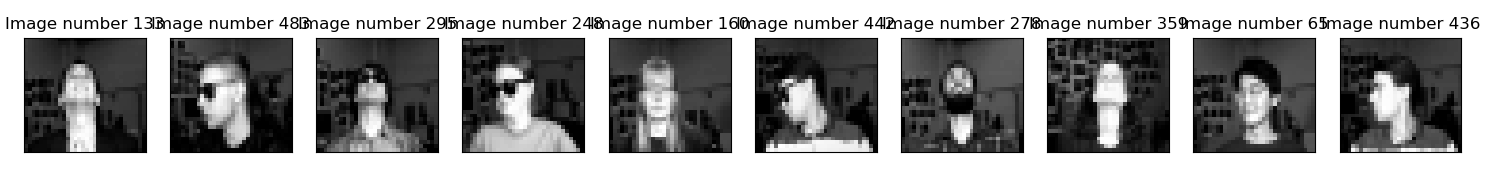
\includegraphics[width=14cm]{2_2_missclassified}
	\caption{}
\end{figure}

\end{document}


%%%%%%%%% end snippet